\TODO{create comparing table, discuss comparing table, review}
% Tabela comparativa das v�rias solu��es
% Analisar e comentar as solu��es
% Introduzir a vossa ideia de solu��o ??

% resumo da sec��o:
In this section we will analyze popular solutions available in the market,
highlighting each solution's strenghts and weaknesses. Later on a table is presented
summarizing each solution and its features. Following that the table is discussed.

\subsection{AutoCAD}
AutoCAD is the \emph{de facto} standard software for architecture designs.
It has a steep learning curve (Figure \ref{FIG-AUTOCAD}) but is learned all over the world and one of
its formats, DXF, is widely supported in 3D modelers and engines. Features
a powerful language, AutoLisp. It favors 2D drawing and modeling but a
skillful operator can create every shape necessary to an architectural scenario.

\begin{figure}[htb]
    \centering
    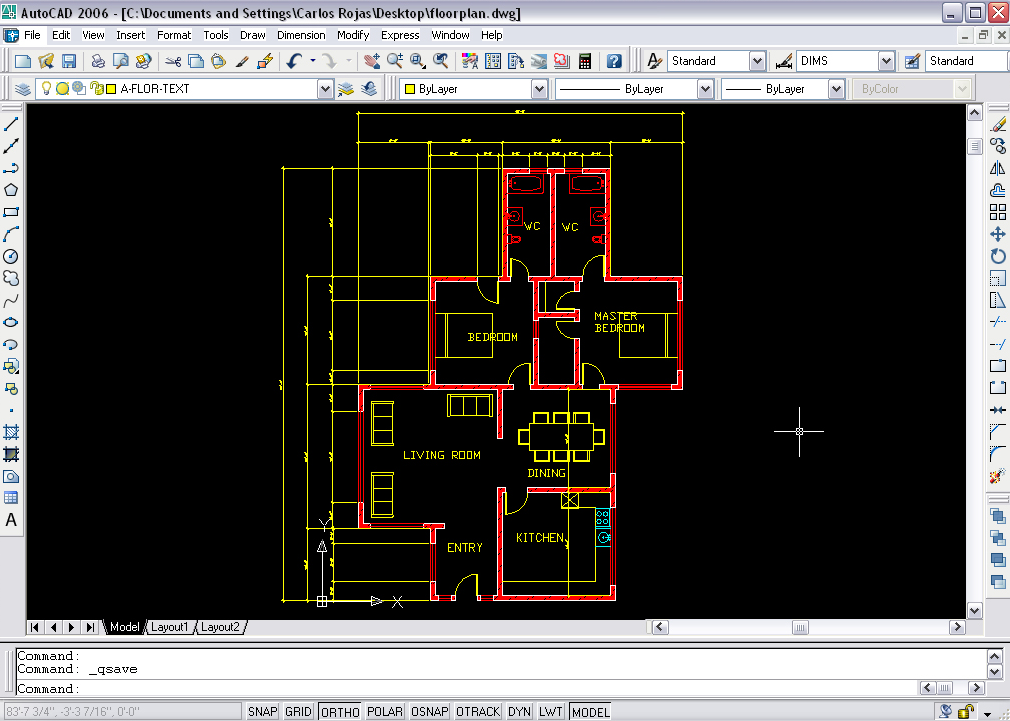
\includegraphics[width=9cm]{gfx/autocad-1.png}
    \caption{AutoCAD: A typical layout of a floor plan.}
    \label{FIG-AUTOCAD}
\end{figure}

\subsection{ArchiCAD}
ArchiCAD aims at conquering new architecture students who haven't been exposed to AutoCAD.
It offers pre-made views and document templates for every architectural driven need.
It is by definition a 3D CAD program and it's praised by architects for its easy 3D manipulations capabilities
(Figure \ref{FIG-ARCHICAD}). Has navigation capabilities too, allowing first person perspective.
Its work flow is thought out to make it easy for an architect to do the most common tasks.
The expressive power to do those extra 10\% uncommon tasks is lacking though.

\begin{figure}[htb]
    \centering
    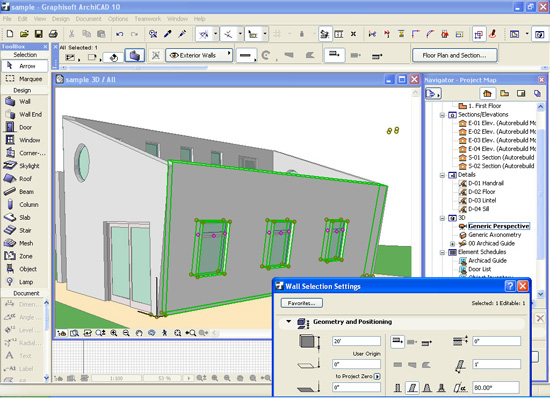
\includegraphics[width=9cm]{gfx/archicad-1.png}
    \caption{ArchiCAD: Notice basic selection and template properties editing in the 3D view.}
    \label{FIG-ARCHICAD}
\end{figure}

\subsection{Revit Building}
Revit Building is another Autodesk product. Unlike AutoCAD, which spans its use to other
areas such as mechanical engineering, Revit Building was explicitly thought out for
architectural design. It works completely in 3D and has native templates for doors,
windows, roofs, etc. There's the concept of mass, lacking in most packages (Figure \ref{FIG-REVIT}).
Being a system for the professional segment, it has a lower learning curve and provides
tools that allow successful modeling of buildings for enthusiasts, something much harder
to do in AutoCAD.

\begin{figure}[htb]
    \centering
    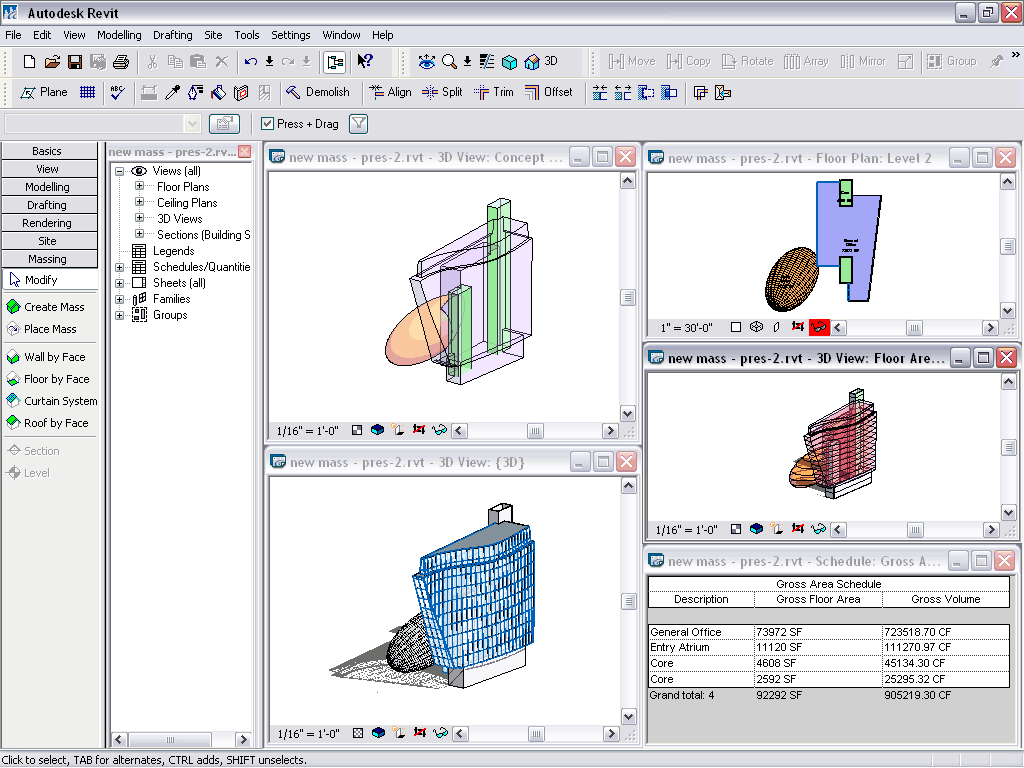
\includegraphics[width=9cm]{gfx/revit-1.png}
    \caption{Revit Building: Solid shapes can be combined with boolean operations and converted into buildings.}
    \label{FIG-REVIT}
\end{figure}

\subsection{SketchUp}
SketchUp is a friendly program for the novice 3D modeler. It features a simple interface
and most of its tools are basic, still able to achieve acceptable results. Its learning curve is great
-- everyone can sketch a room in a nick of time.
Its engine is based on drawing lines on top of lines, the already created surfaces or the construction plane.
It detects the most common geometry restrictions (such as midpoint and perpendicularity).
Features an online repository of models, allowing importing objects such as furniture, trees, props or
well known buildings by just browsing and selection. In awkward angles or when several lines are the 
vicinity of the mouse, strange results occur.
Curve manipulation and generation of surfaces is nonexistent. A great feature of
SketchUp features realtime shadows (Figure \ref{FIG-SKETCHUP}) -- since there's only one viewport, shadows are crucial to
give a sense of depth to a scene. Another bonus from being part of the Google software
library, SketchUp features import/export capabilities to Google Earth. This allows capturing a patch of land
to SketchUp, design a building there and export the patch back with its new contents to Google Earth.

\begin{figure}[htb]
    \centering
    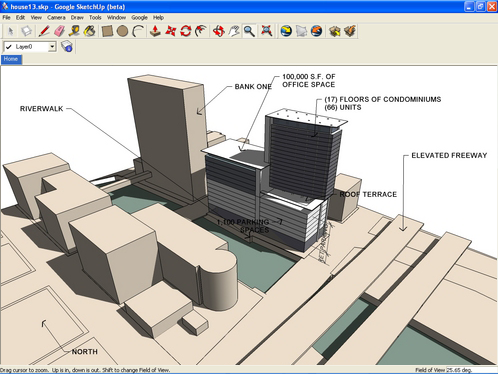
\includegraphics[width=9cm]{gfx/sketchup-1.png}
    \caption{SketchUp: Basic shape extrusions. Notice the shadows in the viewport.}
    \label{FIG-SKETCHUP}
\end{figure}

\subsection{Comparison}
\begin{table}[htb]
    \centering
			\begin{tabular}{|c|c|c|c|c|}
				\hline
				\hline
				% after \\: \hline or \cline{col1-col2} \cline{col3-col4} ...
															& AutoCAD		& ArchiCAD	& Revit Building	& SketchUP	\\
				\hline
				Design in 2D					&			y			&			y			&				y					&			y			\\
				Design in Perspective	&			n			&			+-		&				n					&			y			\\
				%\multispan{5}{|c|}asda\\
				\hline
			\end{tabular}
    \caption{Different solutions in the market compared.}
\end{table}



TODO: discuss the table
